\chapter{Introducción}

\section{Marco teórico}

El BJT se construye con tres regiones semiconductoras separadas por dos uniones pn, como lo muestra la estructura plana epitaxial de la figura 1(a). Las tres regiones se llaman Colector, Base y Emisor En las figuras 1(b) y (c) se
muestran representaciones físicas de los dos tipos de BJT. Un tipo se compone de dos regiones n separadas por una región p (npn) y el otro tipo consta de dos regiones p separadas por una región n (pnp). El término  se refiere al uso tanto de huecos como de electrones como portadores de corriente en la estructura de transistor (Floyd 164).

\begin{figure}[h]
    \centering
    \begin{minipage}[b]{0.32\textwidth}
        \centering
        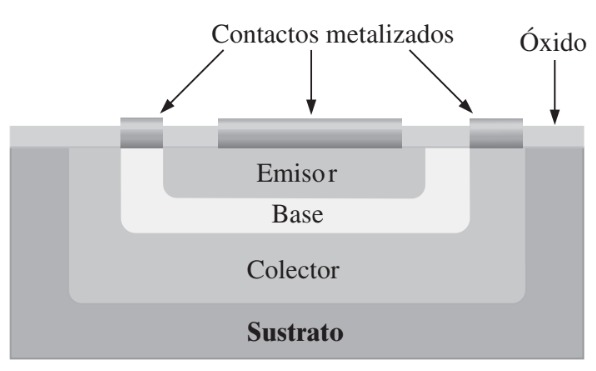
\includegraphics[width=\textwidth]{images/Estructura_plana.jpg}
        \caption*{(a) Estructura plana expitaxial básica}
    \end{minipage}
    \hfill
    \begin{minipage}[b]{0.32\textwidth}
        \centering
        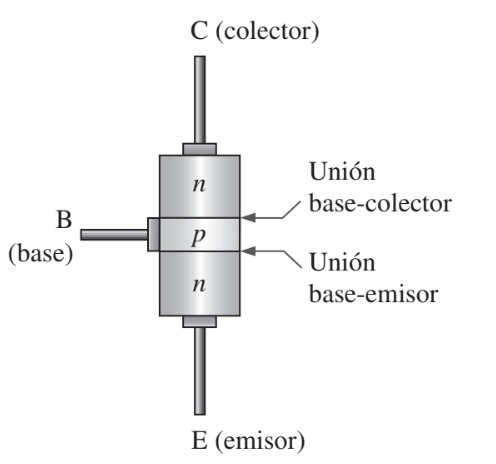
\includegraphics[width=\textwidth]{images/npn.jpg}
        \caption*{(b) npn}
    \end{minipage}
    \hfill
    \begin{minipage}[b]{0.32\textwidth}
        \centering
        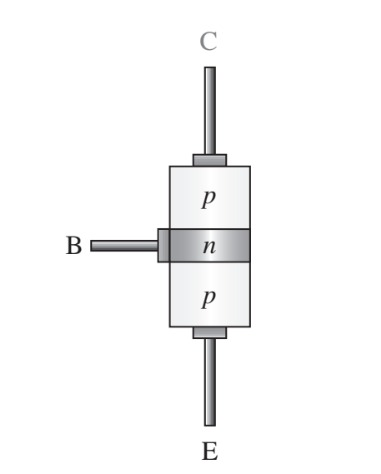
\includegraphics[width=\textwidth]{images/pnp.jpg}
        \caption*{(c) pnp}
    \end{minipage}
    \caption{Construcción básica de un BJT.}
\end{figure}

La unión pn que une la región de la base y la región del emisor se llama unión base-emisor.
La unión pn que une la región de la base y la región del colector se llama unión base-colector, como la figura 1 (b) lo muestra: un conductor conecta a cada una de estas tres regiones. Estos conductores se designan E, B y C por emisor, base y colector, respectivamente. La región de la base está ligeramente dopada y es muy delgada en comparación con las regiones del emisor, excesivamente dopada, y la del colector, moderadamente dopada (la siguiente sección explica la razón de esto).

\section{Operación Básica del BJT}

Para que un BJT opere adecuadamente como amplificador, las dos uniones pn deben estar correctamente polarizadas con voltajes de cd externos. En esta sección se utiliza principalmente el transistor npn como ilustración. La operación del pnp es la misma que para el npn excepto en que los roles de los electrones y huecos, las polaridades del voltaje de polarización y las direcciones de la corriente se invierten.
La figura 2 muestra los arreglos para polarización tanto de BJT npn como pnp para que operen como  Observe que en ambos casos la unión base-emisor (BE) está polarizada en directa y la unión base-colector (BC) polarizada en inversa. Esta condición se llama polarización en directa-inversa.

\begin{figure}[h!]
    \centering
    \begin{minipage}[b]{0.32\textwidth}
        \centering
        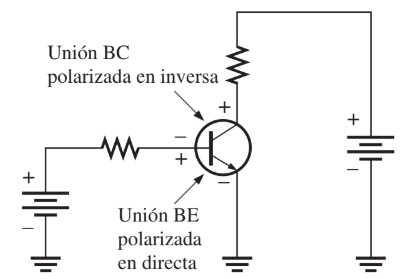
\includegraphics[width=\textwidth]{images/polarizacion_npn.jpg}
        \caption*{(a) npn}
    \end{minipage}
    \hfill
    \begin{minipage}[b]{0.32\textwidth}
        \centering
        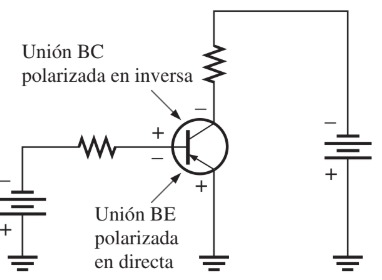
\includegraphics[width=\textwidth]{images/polarizacion_pnp.jpg}
        \caption*{(b) pnp}
    \end{minipage}
    \hfill
    \caption{Polarización del BJT.}
\end{figure}

Para entender cómo opera un transistor, veamos lo que sucede en el interior de la estructura npn. La región del emisor de tipo n excesivamente dopada tiene una densidad muy alta de los electrones de banda de conducción (libres), como muestra la figura 3. Estos electrones libres se difunden con facilidad a través de la unión BE polarizada en directa hacia la región de la base de tipo p muy delgada y levemente dopada (flecha ancha). La base tiene una baja densidad de huecos, los cuales son los portadores mayoritarios, representados por los puntos blancos. Un pequeño porcentaje del número total de electrones libres se va hacia la base, donde se recombinan con huecos y se desplazan como electrones de valencia a través de la base hacia el emisor como corriente de huecos, como lo indican las flechas negras.

\begin{figure}[h]
  \centering
  \begin{minipage}[b]{0.7\textwidth}
    \centering
    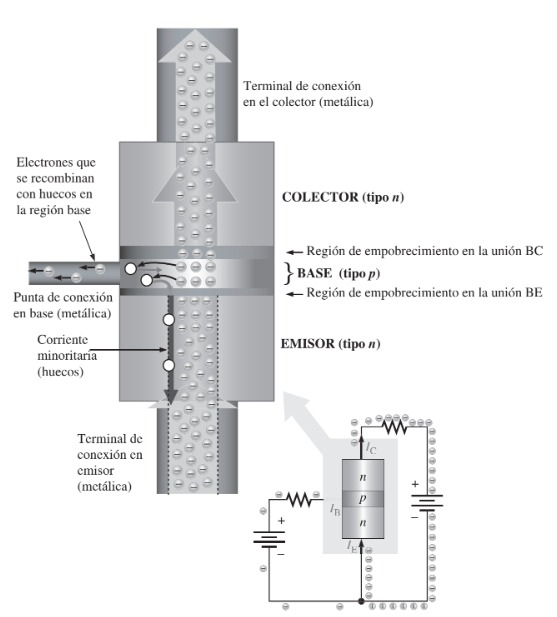
\includegraphics[width=\textwidth]{images/flujo_electrones.jpg}
    \caption{Operacion de un BJT que muestra el flujo de electrones}
  \end{minipage}
  \hfill
\end{figure}

Cuando los electrones que se recombinaron con huecos como electrones de valencia abandonan la estructura cristalina de la base, se transforman en electrones libres en el conductor de la base metálica y producen la corriente de base externa. La mayoría de los electrones libres que entraron a la base no se recombinan con huecos porque es muy delgada. A medida que los electrones libres se desplazan hacia la unión BC polarizada en inversa, son arrastrados a través del colector por la atracción del voltaje de alimentación positivo del colector. Los electrones libres se desplazan a través del colector hacia el circuito externo y luego regresan al emisor junto con la corriente de base, como se indica.
La corriente de emisor es un poco más grande que la corriente de colector debido a la pequeña corriente de base que se desprende de la corriente total inyectada a la base proveniente del emisor.

\newpage
